\documentclass{article}
\usepackage[margin=1.25in]{geometry}
\usepackage{amsmath, amssymb, setspace, enumerate, enumitem}
\usepackage{setspace}
\usepackage{graphicx}
\onehalfspacing

\begin{document}
    \begin{enumerate}
        \item The dimensions of $Z$ are 45
        \item training data:\\
        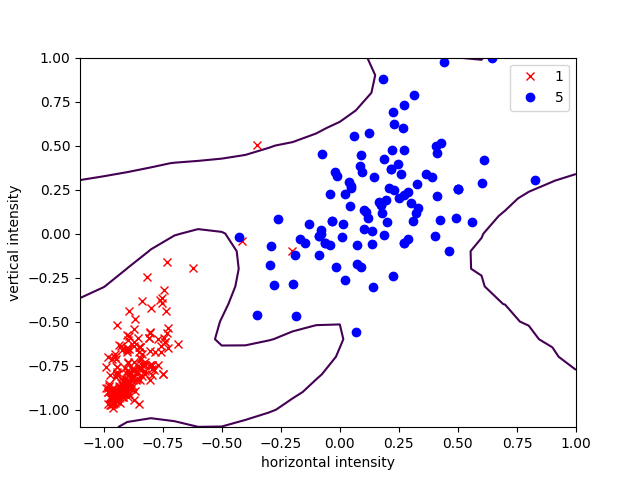
\includegraphics[scale=0.5]{images/reg0train.png}\\
        testing data:\\
        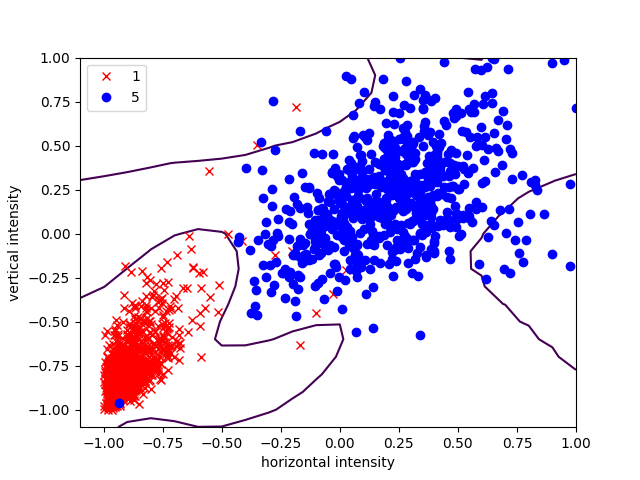
\includegraphics[scale=0.5]{images/reg0test.png}\\
        The data appears to be \textbf{overfitted}
        \item training data:\\
        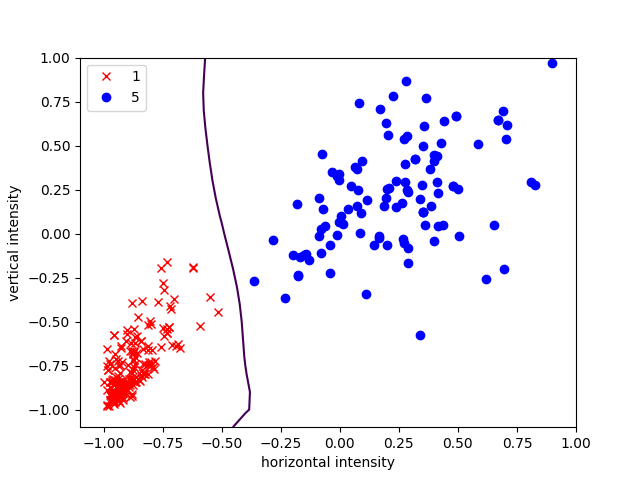
\includegraphics[scale=0.5]{images/reg2train.png}\\
        testing data:\\
        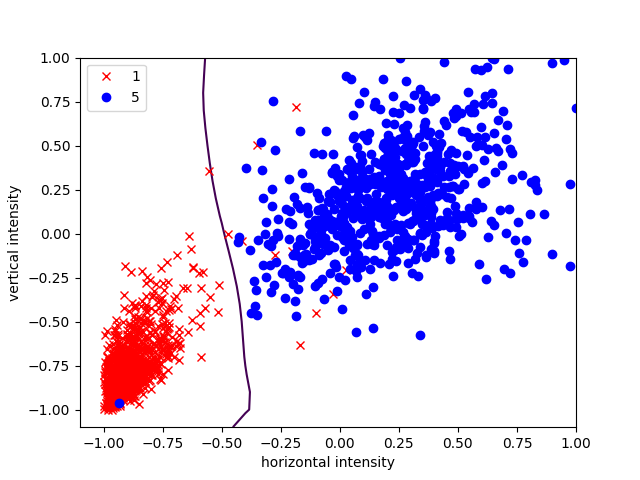
\includegraphics[scale=0.5]{images/reg2test.png}\\
        Data is regularized, there doesn't appear to be any under or overfitting.
        \item Plot:\\ 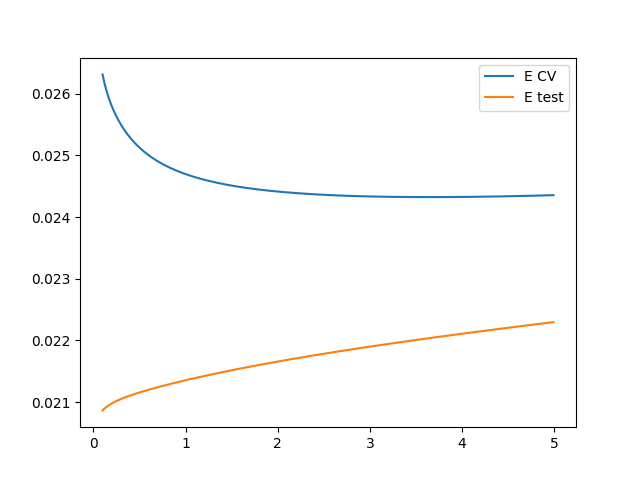
\includegraphics[scale=0.5]{images/CVvsTEST.png}\\
        I chose my values for $\lambda \in \{0, 0.01, 0.02, ..., 5\}$, behavior wise, it appears that as the regularizer increases, the cross validation error decreases, while the regression error onthe test set increases as the regularizer increases.
        \item Plot with $\lambda = 0.57$: \\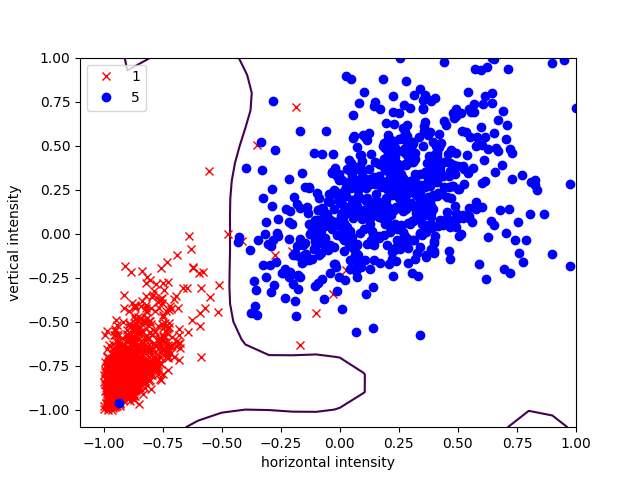
\includegraphics[scale=0.5]{images/bestReg.png}
        \item With regularizer $\lambda = 0.57$, the estimate for out of sample error using $E_{test}(w_{reg}(\lambda ^*))$ is $E_{test} = 0.031$, a good and low rate for an error bar. We can use this to estimate and claim that $E_{out} \approx 0.031$.
        \item No, $E_{cv}$ is an unbiased estimate of $E_{test}$, Despite $E_{cv}$ and $E_{test}$ coming from the same dataset, what is used to determine $E_{cv}$ does not touch on $E_{test}$ at all, so both values don't know about the other.
        \item No, $E_{test}$ is not an unbiased estimate of $E_{out}$, we have used data snooping in the way that we scaled and normalized the entire dataset before separating the training and testing set. This caused the testing set to be affected by the training set in some way because of our normalization, leading to a biased estimate for $E_{out}$.
    \end{enumerate}
\end{document}